%% RSAA THESIS 'TEMPLATE' BY JOSHUA RICH <joshua.rich@gmail.com>
%% README:
% This template is designed to be used with pdflatex rather than plain
% latex.  It was developed under a TeXLive 2007 TeX distribution on
% Linux.  

% for requirements of typesetting and formatting see:
% http://info.anu.edu.au/Policies/_REG/Guidelines/PhD_Exam_Theses.asp
% (in emacs, type M-x browse-url with the cursor on 
% the link above)

%%NOTES ABOUT THE DOCUMENT CLASS
% Yes, I'm using a report style.  Any 'thesis style' you might
% find or someone will give you is based on the standard report
% class, but is probably well outdated compared to whatever TeX
% you have installed.  Besides, why use that style file if you 
% have no idea what it actually does?  You will probably just redefine
% all of its customisations anyway...
\documentclass[11pt,openright]{report} 
\setcounter{secnumdepth}{3}
% define some constants that can be used in various places to easily
% specify title, subjects, author etc.
\newcommand{\thesistitle}{Type Ia Supernovae:
	Explosions and Progenitors}
\newcommand{\fullname}{Wolfgang Eitel Kerzendorf}
\newcommand{\shortname}{W. E. Kerzendorf}
\newcommand{\thesissubjects}{supernova:progenitors ????add some more?????}

%%NOTES ABOUT BABEL PACKAGE:
% It requires two components; the 
% \usepackage line above and the language put in the \documentclass.
% 'british' is used because that is the english style required for an
% ANU thesis.  This will ensure LaTeX uses british hyphenation and
% other language constructs when generating the text.  Putting the
% babel usepackage at the very top also ensures other packages called
% through \usepackage can take advantage of babel if they are set up
% for such.  
% We can also do tricky things in our ~/.emacs file if we
% are an emacs user now as well.  Grab the flyspell-babel and
% ispell-multi  emacs packages from:
% http://www.dur.ac.uk/p.j.heslin/Software/Emacs/
% And put it somewhere Emacs can find it (probably under ~/.emacs.d).
% Then add the following lines to your .emacs:
%   (dolist (hook '(LaTeX-mode-hook))
%   (add-hook hook (lambda () (flyspell-mode 1))))
%   (add-hook 'tex-mode-hook (function (lambda () (setq ispell-parser 'tex))))
%   (autoload 'flyspell-babel-setup "flyspell-babel")
%   (add-hook 'latex-mode-hook 'flyspell-babel-setup)
% After this, you should have Emacs auto-suggesting word corrections
% AND doing it in british-english automagically.  You can do a similar trick
% for papers by simply changing 'british' above to 'american', and
% flyspell will check your paper in american-english.
\usepackage[british]{babel}

%\usepackage{hyperref}

% ---------------------------------------------------------------------
% page size and margins
% ---------------------------------------------------------------------
%%NOTES ABOUT GEOMETRY PACKAGE:
% Below is using the geometry package as it is just cool.  This allows
% you to directly specify the margin requirements as outlined by ANU
% directly.  Here the inner border is 4cm and the outer is 2cm.  Top
% and bottom are also 2cm.  This is much easier than trying to work
% out page and margin dimensions by hand.  This is how you should use
% LaTeX...
\usepackage{geometry}
\geometry{a4paper,twoside}
\geometry{includehead,includefoot}
\geometry{hmargin={4cm,2cm}}
\geometry{vmargin={2cm,2cm}}

% ---------------------------------------------------------------------
% miscellaneous packages used
% ---------------------------------------------------------------------
\usepackage[hiresbb]{graphicx}
\DeclareGraphicsExtensions{.pdf}
%\DeclareGraphicsExtensions{.eps}
\usepackage[twoside]{rotating}

%%NOTES ABOUT FONTS PACKAGES:
% The basic requirements for fonts in an ANU thesis demand clear
% readability and that is about all.  So if you choose a nice,
% standard serif font you won't have any problems.
% I several font families in my thesis below:
%  pxfonts: math typesetting
%  tgpagella: for the normal text font (serif)
%  tgheros: for the sans serif font
%  tgcursor: for the typewriter style font
% TeX Gyre Pagella, Heros and Cursor are part of the TeX Gyre family
% of fonts, which can be obtained from:
%   http://www.gust.org.pl/projects/e-foundry/tex-gyre/
% Not all of the TeX Gyre, and possibly not the latest glyphs are
% available in standard TeX distributions.  
%
% The 'mathpazo' package provides an almost identical, albeit not
% actively developed font family to TeX Gyre Pagella and is included
% in standard TeX distributions.  This package
% also provides a full range of math glyphs.  You'd need to find
% alternative sans serif and typewriter fonts to use with this package.
%
% You can see a whole heap of LaTeX fonts, most of which are also in a
% standard TeX distribution at: 
%  http://www.tug.dk/FontCatalogue/
% This web-page shows what each font looks like and what you need to
% do to include the font in your document.  Note it lists fonts that
% may not be installed by your default TeX installation...
%
% Another list of fonts, recommended by `typophiles' can be found at:
%  http://typophile.com/node/18207
% Although the above list includes some really nice fonts, their
% availability in TeX distributions varies.  You may have to install
% them manually...
\usepackage[T1]{fontenc}
\usepackage{textcomp}
\usepackage{ucs}
\usepackage[utf8x]{inputenc}
\usepackage{amsmath,amssymb}
\usepackage{pxfonts}
\usepackage{tgheros,tgpagella}
\renewcommand*\ttdefault{qcr}
\linespread{1.05} % tgpagella/mathpazo need a bigger line spacing
\usepackage{microtype}
% bibliography uses natbib, this will be a requirement
\usepackage[round]{natbib}
% Super-nice looking tables, better than deluxetable
\usepackage{longtable,booktabs,multirow,ctable}
%\usepackage{deluxetable}

%%NOTES ABOUT CAPTION AND SUBFIG PACKAGES
% I'm using the caption package to style my captions.
% You need to read the documentation for this package (on CTAN) as it
% has simple explanations of the options and examples of what it looks
% like.
%
% The subfig package allows the ability to control in detail
% positioning of sub-plots in a complex figure as well as add labels
% to them, which can then be referenced in the text without the need
% for changing the actual number as your sub-figures change.
% The subfig package inherits options from the caption package, so
% declare them together.
%
\usepackage[]{caption,subfig}
\captionsetup{format=hang,%
  indention=-1.5cm,%
  labelsep=quad,%
  labelfont={footnotesize,bf},%
  textfont={footnotesize}}
% The hyperref package is a must while editing.  It provides urls
% inside your document; you can then click to go to certain pages,
% figures or bibliography entries.
\usepackage[unicode,pageanchor,colorlinks,plainpages=false]{hyperref}
% \hypersetup{pdftitle=\thesistitle\ - \shortname,%
%   pdfauthor=\fullname,%
%   pdfsubject={\thesissubjects},%
%   citecolor=DodgerBlue3,%
%   linkcolor=Ivory4,%
%   anchorcolor=CadetBlue4}
%for printing, make all colours black...
\hypersetup{pdftitle=\thesistitle\ - \shortname,%
pdfauthor=\fullname,%
pdfsubject={\thesissubjects},%
%citecolor=green,%
%filecolor=blue,%
%linkcolor=blue,%
%urlcolor=blue%
}
% Drop capitals at the start of chapters
\usepackage{lettrine}
% Allow defining of colours. Useful for:
% - defining the colours of links, citations etc.
% together with hyperref (i.e. in hyperrefsetup)
% - get alternating row colours or shades in tables
\usepackage[hyperref,x11names]{xcolor}
% Stops figures and tables 'floating' past the section in which they
% are declared.
\usepackage[section]{placeins}
\usepackage[toc,page,title,title]{appendix}
%%NOTES ABOUT NAG
% this is a very good package to use.  If you want to write good LaTeX
% code and want to make sure you aren't using outdated methods (like
% your supervisor does), then use this package.  It will complain when
% you use outdated or wrong LaTeX commands.
\usepackage[l2tabu, orthodox]{nag}
\usepackage{ifthen}

% ---------------------------------------------------------------------
% styles for header, footer, pages, bibliography
% ---------------------------------------------------------------------
%

% chapter heading style
% this is the 'Conny' style from the fncychap package, modified to
% remove the two bold lines before the 'Chapter X' title.
% For usage of this package, see:
%  http://tug.ctan.org/cgi-bin/ctanPackageInformation.py?id=fncychap
%
\usepackage{fncychap}
\makeatletter
\ChNameUpperCase
\ChTitleUpperCase  
\ChNameVar{\centering\Huge\usefont{OT1}{qbk}{m}{n}\selectfont}
\ChNumVar{\Huge}
\ChTitleVar{\centering\Huge\usefont{OT1}{qbk}{m}{n}\selectfont}
\ChRuleWidth{2pt}
\renewcommand{\DOCH}{%
  \CNV\FmN{\@chapapp}\space \CNoV\thechapter
  \par\nobreak
  \vskip -0.5\baselineskip
}
\renewcommand{\DOTI}[1]{%
  \mghrulefill{\RW}\par\nobreak
  \CTV\FmTi{#1}\par\nobreak
  \vskip 60\p@
}
\renewcommand{\DOTIS}[1]{%
  \mghrulefill{\RW}\par\nobreak
  \CTV\FmTi{#1}\par\nobreak
  \vskip 60\p@
}

%
%%% page styles:
%
\usepackage{fancyhdr}
\fancyhead{}
\fancyfoot{}
%% make the odd pages have the section name on the top right
%\fancyhead[RO]{\usefont{OT1}{qbk}{m}{n}\selectfont \rightmark}
%% make the even pages have the chapter name on the top left
%\fancyhead[LE]{\usefont{OT1}{qbk}{m}{n}\selectfont \leftmark}
%
% fancy (main content) page header/footer styles
\fancyfoot[LE]{\usefont{OT1}{qbk}{m}{n}\selectfont \thepage}
\fancyfoot[RO]{\usefont{OT1}{qbk}{m}{n}\selectfont \thepage}
\renewcommand{\footrulewidth}{0.5pt}
\renewcommand{\footruleskip}{0mm}
% plain page header/footer styles (i.e. chapter pages)
\fancypagestyle{plain}{
\fancyhf{}
\fancyfoot[LE]{\usefont{OT1}{qbk}{m}{n}\selectfont \thepage}
\fancyfoot[RO]{\usefont{OT1}{qbk}{m}{n}\selectfont \thepage}
\renewcommand{\headrulewidth}{0pt}
\renewcommand{\footrulewidth}{0pt}
}

%
% this next section (till \makeatother) makes sure that blank pages
% are actually completely blank, cause they're not usually
\makeatletter
\def\cleardoublepage{\clearpage\if@twoside \ifodd\c@page\else
	\hbox{}
	\vspace*{\fill}
	\thispagestyle{empty}
	\newpage
	\if@twocolumn\hbox{}\newpage\fi\fi\fi}
\makeatother

%
%%% section header styles:
%
\usepackage[calcwidth]{titlesec}
\titlelabel{\thetitle.\quad}


%\includeonly{macros,chapter1}
%\includeonly{macros,chapter2}
%\includeonly{macros,chapter3}
%\includeonly{macros,chapter4}

% uncomment if you would like an index (make sure you actually define
% index terms in your document as well...
\makeindex

% this contains various command definitions and other misc. options
% ---------------------------------------------------------------------
% command re-definitions and additions
% ---------------------------------------------------------------------

% i.e. -- e.g. -- etc. -- et. al.
\newcommand{\eg}{{\em e.g.,}}
\newcommand{\ie}{{\em i.e.,}}
\newcommand{\etc}{{\em etc.}}
\newcommand{\etal}{{\em et al.}}

% symbols
\newcommand{\HI}{\hbox{\rmfamily H\,{\textsc i}}}
\newcommand{\HIfat}{\hbox{\rmfamily\bfseries H\,{\textsc i}}}
\newcommand{\HIsub}{\hbox{{\scriptsize H}\,{\tiny I}}}
\newcommand{\HII}{\hbox{\rmfamily H\,{\scshape ii}}}
\newcommand{\HIIsub}{\hbox{\scriptsize \rmfamily H\,{\scshape ii}}}
\newcommand{\Ha}{\hbox{\rmfamily H\,$\alpha$}}
\newcommand{\msun}{\hbox{$M_{\odot}$}}
\newcommand{\mhi}{\hbox{$M_{\HIsub}$}}
\newcommand{\lsun}{\hbox{$L_{\odot}$}}
\newcommand{\mlsun}{(M/L)_{\odot}}
\newcommand{\vexp}{\hbox{$V_{exp}$}}
\newcommand{\vhel}{\hbox{$V_{hel}$}}
\newcommand{\vdisp}{\hbox{$\sigma_{disp}$}}
\newcommand{\Nhi}{\hbox{$N_{\HIsub}$}}
\newcommand{\nhi}{\hbox{$n_{\HIsub}$}}
\newcommand{\Mhi}{\hbox{$M_{\HIsub}$}}
\newcommand{\ra}{$\alpha$}
\newcommand{\dec}{$\delta$}
\newcommand{\degree}{\textdegree}
\newcommand{\arcmin}{\hbox{$^\prime$}}
\newcommand{\arcsec}{\hbox{$^{\prime\prime}$}}
\newcommand{\kms}{\hbox{km s$^{-1}$}}
\newcommand{\mjbeam}{\hbox{mJy beam$^{-1}$}}
\newcommand{\jbeam}{\hbox{Jy beam$^{-1}$}}
\newcommand{\mjbeamkms}{\hbox{mJy/beam km s$^{-1}$}}
\newcommand{\jkms}{\hbox{Jy km s$^{-1}$}}
\newcommand{\coldensity}{\hbox{cm$^{-2}$}}
\newcommand{\voldensity}{\hbox{cm$^{-3}$}}
% add others you need

% footnote symbols
% use \symbolfootnote[1]{footnote} to get an *
%     * 1 - *
%     * 2 - dagger
%     * 3 - double dagger
%     * 4 - ... 9 (see page 175 of the latex manual) 
\long\def\symbolfootnote[#1]#2{\begingroup%
\def\thefootnote{\fnsymbol{footnote}}\footnote[#1]{#2}\endgroup}
% New definition of square root:
% it renames \sqrt as \oldsqrt
% it defines the new \sqrt in terms of the old one
% See:
%  http://en.wikibooks.org/wiki/LaTeX/Tips_and_Tricks#New_Square_Root
\let\oldsqrt\sqrt
\def\sqrt{\mathpalette\DHLhksqrt}
\def\DHLhksqrt#1#2{%
\setbox0=\hbox{$#1\oldsqrt{#2\,}$}\dimen0=\ht0
\advance\dimen0-0.2\ht0
\setbox2=\hbox{\vrule height\ht0 depth -\dimen0}%
{\box0\lower0.4pt\box2}}
% define a new url command so a nice font can be used
\newcommand{\myurl}[1]{\small\texttt{#1}}
% handy referencing of figures/tables, see 'Guide to using Encapsulated
% PostScript in LaTeX.', Section 17.1.1
\newcommand\FigDiff[1]{\hyperref[#1]{Figure~\ref*{#1}} on Page~\pageref*{#1}}
\newcommand\FigSame[1]{\hyperref[#1]{Figure~\ref*{#1}}}
\newcommand\Figref[1]{\ifthenelse{\value{page}=\pageref{#1}}
                     {\FigSame{#1}}{\FigDiff{#1}}}
\newcommand\TabDiff[1]{\hyperref[#1]{Table~\ref*{#1}} on Page~\pageref*{#1}}
\newcommand\TabSame[1]{\hyperref[#1]{Table~\ref*{#1}}}
\newcommand\Tabref[1]{\ifthenelse{\value{page}=\pageref{#1}}
                     {\TabSame{#1}}{\TabDiff{#1}}}

% text to add to end of continued figures caption
\newcommand\ContFig[1]{\textit{(Figure continued from page \pageref*{#1})}}

% ---------------------------------------------------------------------
% pdflatex setup
% ---------------------------------------------------------------------
% make pdflatex use the same spacing (paragraph, line and page breaks)
% as standard LaTeX 
\pdfadjustspacing=1

% ---------------------------------------------------------------------
%  misc. options
% ---------------------------------------------------------------------
% table of contents will go to subsubsections
\setcounter{tocdepth}{3}  

% ---------------------------------------------------------------------
% more liberal 'float' (tables, figures) placement
% ---------------------------------------------------------------------
% Alter some LaTeX defaults for better treatment of figures:
% See p.105 of "TeX Unbound" for suggested values.
% See pp. 199-200 of Lamport's "LaTeX" book for details.
% General parameters, for ALL pages:
\renewcommand{\topfraction}{0.9}	% max fraction of floats at top
\renewcommand{\bottomfraction}{0.8}	% max fraction of floats at bottom
% Parameters for TEXT pages (not float pages):
\setcounter{topnumber}{2}
\setcounter{bottomnumber}{2}
\setcounter{totalnumber}{4}     % 2 may work better
\setcounter{dbltopnumber}{2}    % for 2-column pages
\renewcommand{\dbltopfraction}{0.9}	% fit big float above 2-col. text
\renewcommand{\textfraction}{0.07}	% allow minimal text w. figs
% Parameters for FLOAT pages (not text pages):
\renewcommand{\floatpagefraction}{0.7}	% require fuller float pages
% N.B.: floatpagefraction MUST be less than topfraction !!
\renewcommand{\dblfloatpagefraction}{0.7}	% require fuller float pages
% remember to use [htp] or [htpb] for placement

% ---------------------------------------------------------------------
% Journal name abbreviations
% ---------------------------------------------------------------------
\newcommand{\jnlref}[1]{\textrm{#1}}
\newcommand{\aj}{\jnlref{AJ}}
\newcommand{\araa}{\jnlref{ARA\&A}}
\newcommand{\apj}{\jnlref{ApJ}}
\newcommand{\apjl}{\jnlref{ApJ}}
\newcommand{\apjs}{\jnlref{ApJS}}
\newcommand{\ao}{\jnlref{Appl.~Opt.}}
\newcommand{\apss}{\jnlref{Ap\&SS}}
\newcommand{\aap}{\jnlref{A\&A}}
\newcommand{\aapr}{\jnlref{A\&A~Rev.}}
\newcommand{\aaps}{\jnlref{A\&AS}}
\newcommand{\azh}{\jnlref{AZh}}
\newcommand{\baas}{\jnlref{BAAS}}
\newcommand{\jrasc}{\jnlref{JRASC}}
\newcommand{\memras}{\jnlref{MmRAS}}
\newcommand{\mnras}{\jnlref{MNRAS}}
\newcommand{\pra}{\jnlref{Phys.~Rev.~A}}
\newcommand{\prb}{\jnlref{Phys.~Rev.~B}}
\newcommand{\prc}{\jnlref{Phys.~Rev.~C}}
\newcommand{\prd}{\jnlref{Phys.~Rev.~D}}
\newcommand{\pre}{\jnlref{Phys.~Rev.~E}}
\newcommand{\prl}{\jnlref{Phys.~Rev.~Lett.}}
\newcommand{\pasp}{\jnlref{PASP}}
\newcommand{\pasj}{\jnlref{PASJ}}
\newcommand{\qjras}{\jnlref{QJRAS}}
\newcommand{\skytel}{\jnlref{S\&T}}
\newcommand{\solphys}{\jnlref{Sol.~Phys.}}
\newcommand{\sovast}{\jnlref{Soviet~Ast.}}
\newcommand{\ssr}{\jnlref{Space~Sci.~Rev.}}
\newcommand{\zap}{\jnlref{ZAp}}
\newcommand{\nat}{\jnlref{Nature}}
\newcommand{\iaucirc}{\jnlref{IAU~Circ.}}
\newcommand{\aplett}{\jnlref{Astrophys.~Lett.}}
\newcommand{\apspr}{\jnlref{Astrophys.~Space~Phys.~Res.}}
\newcommand{\bain}{\jnlref{Bull.~Astron.~Inst.~Netherlands}}
\newcommand{\fcp}{\jnlref{Fund.~Cosmic~Phys.}}
\newcommand{\gca}{\jnlref{Geochim.~Cosmochim.~Acta}}
\newcommand{\grl}{\jnlref{Geophys.~Res.~Lett.}}
\newcommand{\jcp}{\jnlref{J.~Chem.~Phys.}}
\newcommand{\jgr}{\jnlref{J.~Geophys.~Res.}}
\newcommand{\jqsrt}{\jnlref{J.~Quant.~Spec.~Radiat.~Transf.}}
\newcommand{\memsai}{\jnlref{Mem.~Soc.~Astron.~Italiana}}
\newcommand{\nphysa}{\jnlref{Nucl.~Phys.~A}}
\newcommand{\physrep}{\jnlref{Phys.~Rep.}}
\newcommand{\physscr}{\jnlref{Phys.~Scr}}
\newcommand{\planss}{\jnlref{Planet.~Space~Sci.}}
\newcommand{\procspie}{\jnlref{Proc.~SPIE}}
\newcommand{\ieeesigprocm}{\jnlref{IEEE~Signal~Processing~Magazine}}
\newcommand{\cjaa}{\jnlref{Chinese J. Astron. Astrophys.}}
\let\astap=\aap
\let\apjlett=\apjl
\let\apjsupp=\apjs
\let\applopt=\ao

%%% Local Variables:
%%% TeX-master: "thesis.tex"
%%% End:


\begin{document}
%\tableofcontents \newpage
% !TEX root = ../thesis.tex
\chapter{Progenitor search in SN 1006}
\label{chap:sn1006}


\section{Introduction}

The search for a donor star in \sn{1572}{}\ has not turned up an obvious candidate. However, we have detected two objects (\starb\ and \starg) exhibiting some unusual properties, which while interesting, ultimately seem inconsistent with the expectations of any viable donor star scenario. \Gls{donor} star scenarios are theoretical in their nature and any actual donor star is likely to not exhibit all features predicted by the model. Therefore, we have reached an impasse with \sn{1572}{} and more detailed observations will likely not provide a definitive answer if either of these two stars were involved in the progenitor system. An obvious way forward is to scrutinise stars in other \snia\ remnants and see if any of those have similar properties to \starb\ or \starg. The remnant of \sn{1006}{} is the ideal object for this kind of follow-up search. 

The lack of a central neutron star, observation of several tenths of a solar mass of iron inside the remnant \citep{1997ApJ...481..838H} and the the high peak luminosity and basic light curve shape \citep[visible for several years][]{1965AJ.....70..748G} all indicate that \sn{1006}{} was a \snia. The remnant has a secure distance, measured by \citet{2003ApJ...585..324W}, who combined the proper motion and the radial velocity of the expanding shell to measure the distance to 2.2~\kpc, making \sn{1006}{} the closest of the ancient \snia\ remnants (consistent \sn{1006}{} being the brightest).   The geometric centre of the remnant is well determined from both \xray\ and radio observations \citep{2003ApJ...585..324W}. In addition, the interior of the remnant has been probed with UV background sources \citep{2005ApJ...624..189W}. 

This revealed the aforementioned iron core as well as a silicon-rich shell. The remnant has been searched for possible objects associated with the supernova explosion previously, and an unusual O-star had been identified as a possible donor star to \sn{1006}{}. This unusual O-Star was identified near the centre of \sn{1006}{} by \citet{1980ApJ...241.1039S} and is now called Schweizer-Middleditch Star (\smstar). After successful identifications of neutron stars in both the Vela Remnant and the Crab Remnant this was thought to be the third identification of a stellar remnant in a historical supernova. Subsequent UV spectroscopic follow-up of the \smstar\ by \citet{1983ApJ...269L...5W}, showed strong \ion{Fe}{2} lines with a profile broadened by a few thousand \kms. In addition, \citet{1983ApJ...269L...5W} identified redshifted \ion{Si}{2}, \ion{Si}{3} and \ion{Si}{4} lines. Their conclusion was that these absorption lines stem from the remnant and place the \smstar\ behind the remnant, making it unrelated to \sn{1006}{}. Although unrelated, the \smstar\ is an ideal object to probe the remnant and measure upper limits for interstellar extinction \citep[E(B-V) = 0.1][]{1993ApJ...416..247W,2003ApJ...585..324W}.


SN 1006 has several properties which make it well suited to undertake a progenitor search.  Although the remnant is the oldest among the known \snia\ remnants, its age is still young enough that  the remnant's centre is well determined, and the motion of any potential donor star low enough that only a small area of stars need to be searched. Furthermore, this elapse of 1005 years is a short length of time relative to the timescales of stellar evolution for donor stars \cite[see][]{2000ApJS..128..615M} - we still expect a potential donor star to be close to the same state as directly after the supernova explosion. In addition, \sn{1006}{} has a low interstellar extinction, which eases the determination of stellar parameters. These serendipitous conditions for the \sn{1006}{} remnant led us to launch a photometric and spectroscopic campaign to search for the donor star. Our photometric observations were taken at Siding Spring Observatory with the 2.3m Telescope imager. The spectroscopic observations were undertaken with the high resolution multi-object spectrograph \gls{flames} attached to the \gls{vlt}.


In Section \ref{sec:obs_red} we outline the observations as well as data reduction of the photometric and spectroscopic data. Section \ref{sec:sn1006_analysis} is split into four subsections, namely radial velocity, stellar rotation and stellar parameters. We conclude this chapter in Section \ref{sec:sn1006:conclusion} and discuss the possible implications of our initial find as well as outlining some future work.


\section{Observations and Data Reduction}
\label{sec:obs_red}
\subsection{Photometric Observations}
\Gls{ccd} images of \sn{1006}{} were obtained using the imaging camera at the Nasmyth-B focus of the ANU 2.3~m Telescope at
the Siding Spring Observatory, on 11 May 2004. We exposed for 1860~s in U-Band, 1490~s in B-Band, 788~s in V-Band and 1860~s in I-Band. For calibration purposes we took images of the PG1633 and PG1047 standard star regions in the same filters. The seeing ranged between 1\arcsec and 2\arcsec, and the conditions were photometric. 
The data were bias corrected and flatfielded (using skyflats) using \gls{pyraf}.

For our photometric data reduction we fitted an astrometric solution using astrometry from the \twomass\ point source catalogue \citep{2006AJ....131.1163S} to our frames. 
We used \gls{sextractor} to measure the magnitudes of the objects in the frames and then calibrated our photometry to a standard Bessell Filter system using the Stetson magnitudes \footnote{This research used the facilities of the Canadian Astronomy Data Centre operated by the National Research Council of Canada with the support of the Canadian Space Agency} of our standard fields PG1633 and PG1047 .  

The measured magnitudes were supplemented with near infrared magnitudes from the \twomass\ point source catalogue (see Table \ref{tab:sn1006_twomass} and \ref{tab:sn1006_photometry} ). Subsequently we checked the photometric measurements, by plotting the obtained $B-V$ colours against the $V-K$ colours (see Figure \ref{fig:colour_check}).
\begin{figure}[htbp] %  figure placement: here, top, bottom, or page
   \centering
   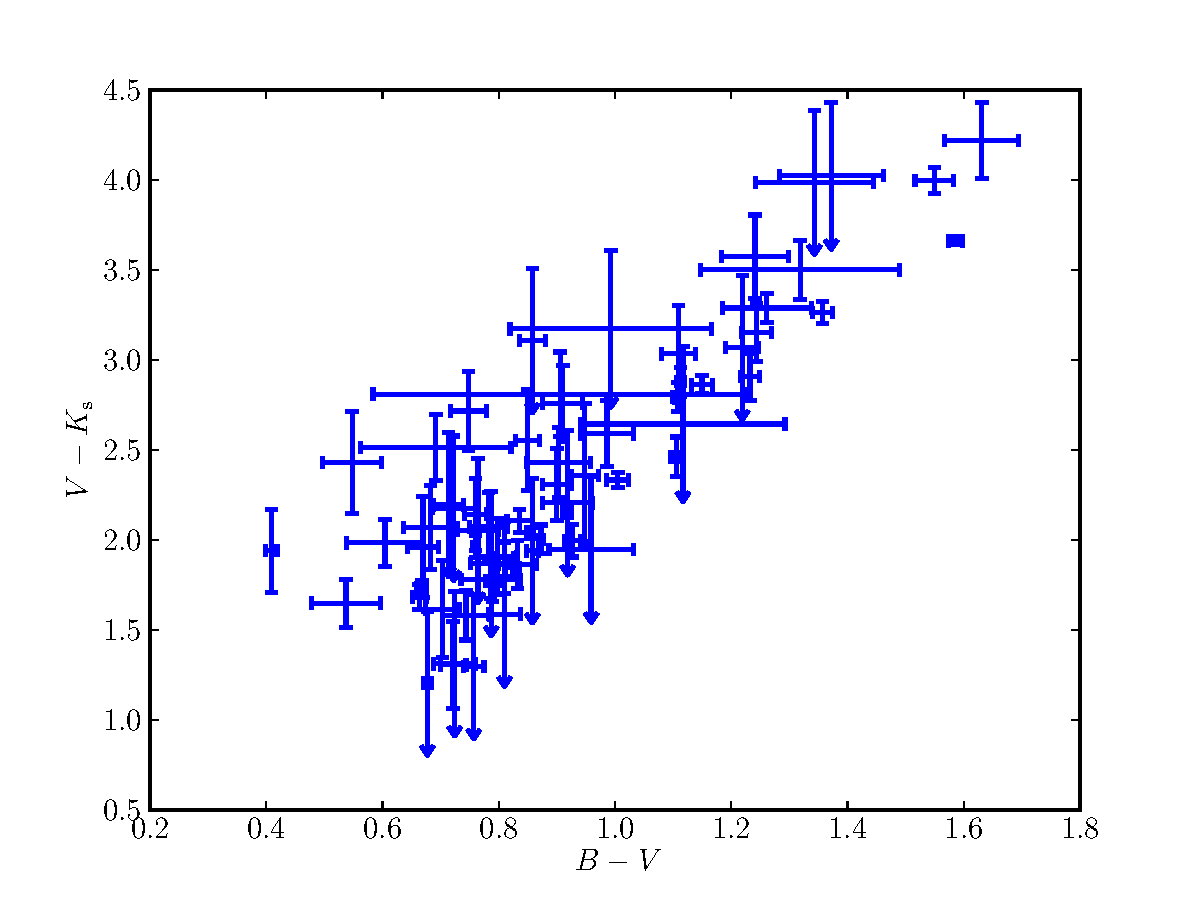
\includegraphics[width=\textwidth]{chapter_sn1006/plots/color_bv_vk.pdf} 
   \caption[Colour-colour plot of all candidates in SN 1006 to check photometry]{Colour-colour plot of all candidates in SN 1006 to check photometry. The correspondence is as expected given the uncertainties in the measurements.}
   \label{fig:colour_check}
\end{figure}

We have also computed temperatures from photometric colours by using the polynomials given in \citet{2010A&A...512A..54C}. In the first instance, we assumed a solar \gls{feh} for all stars, but the choice of \gls{feh} only has a minor influence on the temperature calculation (e.g. change of 300K between \feh=0 and \feh=-1) for the temperature. In addition, the temperature polynomial coefficients incorporating the metallicity are particularly small for the $V-K$ colour. All temperatures are listed in the optical photometry Table \ref{tab:sn1006_photometry} and infrared photometry Table \ref{tab:sn1006_twomass}.


\subsection{Spectroscopic Observations}

For the spectroscopy survey we used the \gls{vlt} instrument \gls{flames}, which can provide high resolution (R=25,000) optical spectra over a 25\arcmin\ field of view for up to 130 objects. In this mode, the spectral coverage is limited to 200~\AA, and we chose the wavelength region from 5139~\AA\ to 5356~\AA\ which contains the gravity sensitive \gls{mgb} Triplet as well as many iron lines to accurately measure metallicity. For the centre of our spectroscopic survey we chose the mean of the \xray\ and radio centre \citep[\rasc{15}{02}{22}{1}\ \decl{-42}{05}{49};][]{2003ApJ...585..324W}. We chose a search radius of 120\arcsec\ - corresponding to the motion of a star travelling 1250~\kms at 2.2~\kpc\ over 1000 years. This generous choice, which is more than four times our maximum expected escape velocity (see Figure \vref{fig:han2008_vrad}), was made to accommodate any errors in the choice of the centre. Although the models predict the surviving companion to be several hundred \lsun\ \citep{2000ApJS..128..615M}, we chose a limiting magnitude of $V=17.5$ ($0.5~\lsun(V)$ at 2.2~\kpc\ including extinction of E(B-V)=0.1) to accommodate a wide range of potential \gls{donor} stars. An exposure time of 3.8~hours was chosen to obtain spectra with high enough quality to measure rotation and basic stellar parameters (\snratio\ $>20$). For completeness and to not waste fibres we chose additional stars down to a magnitude limit of $V=19$, which are only used for radial velocity measurements. These constraints yielded 26 stars with $V<17.5~\textrm{mag}$ and 53 stars in the bin between $17.5<V<19~\textrm{mag}$ (for a total of 79 stars) for our survey (see Figure \ref{fig:overview_sn1006}). With fibre buttons not being able to be placed less than 11\arcsec\ apart, we had to split our candidates over three different setups. The first two setups were observed five times with 2775~seconds each. We deliberately chose bright stars for the last setup so that it only had to be observed three times with 2775 s each. In addition, we placed spare fibres on three bright stars (R$\approx 10$; 2MASS J15032744-4204463, 2MASS J15031746-4204165, 2MASS J15033195-4202356) located close to the edge of the 25\arcmin\ field of view for calibration purposes. Additional spare fibres were placed on sky positions, which were chosen to be far from \twomass\ sources and manually inspected on DSS images to be in star free regions.
\begin{figure}[tb] %  figure placement: here, top, bottom, or page
   \centering
   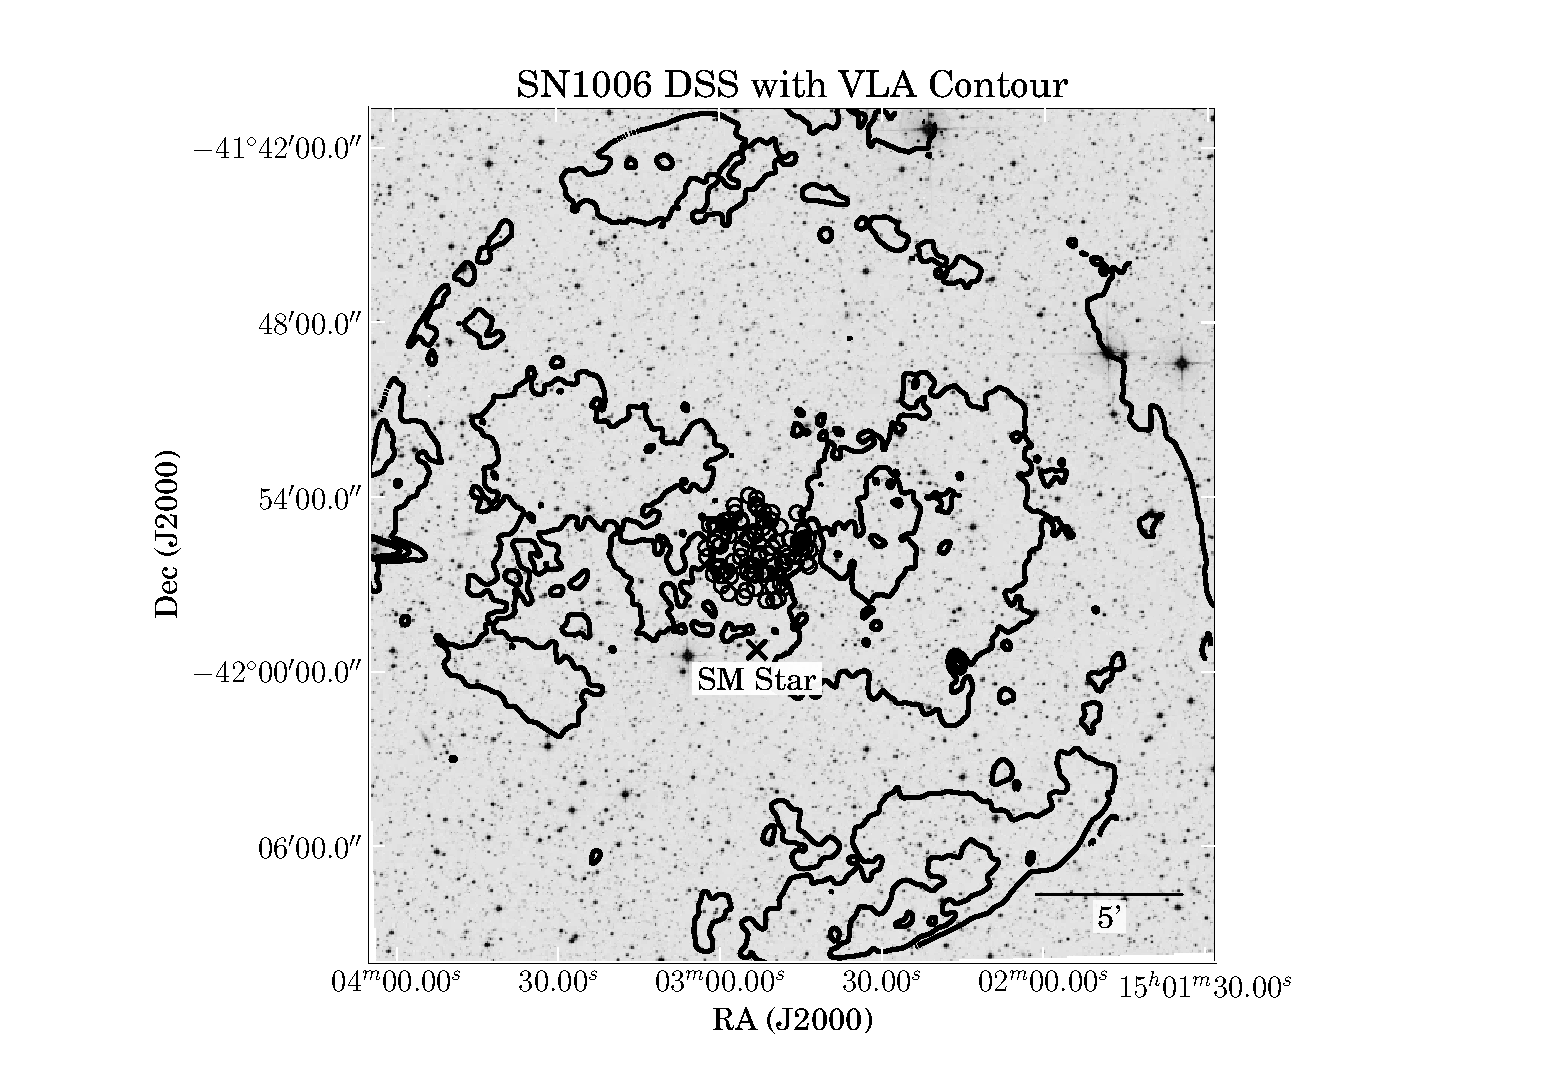
\includegraphics[width=\textwidth, trim=2cm 0 4cm 0, clip]{chapter_sn1006/plots/sn1006_overlay_withsm.pdf} 
   \caption[Overview of candidates and remnantin SN 1006]{Optical DSS image with radio contour overlay (VLA). The black circles in the centre show the 79 program stars. Additionally we have marked the `spurious` donor the \smstar.}
   \label{fig:overview_sn1006}
\end{figure}
In addition, to our night time calibration, which included simultaneous arc exposures with four fibres for each observation block, we received standard daytime calibrations. In total, 13 observation blocks with an exposure time of 2775~seconds each were obtained. Table \ref{tab:observations} provides the Observing ID, modified julian date, mean seeing, mean airmass, setup name and heliocentric correction for all observations (all data is available under ESO Program ID: 083.D-0805(A)). Due to broken fibres, not all stars where observed for the expected length of time. Broken fibres caused \candstar{31} not to be observed at all in this project (see Figure \ref{fig:sn1006:zoomed_overview}) - although a $V=17.87~\textrm{mag}$ is not part of our primary sample.
\begin{deluxetable}{cccccc}
\tablecaption{Observations}
\tablehead{\colhead{ObsID} & \colhead{MJD} & \colhead{FWHM} & \colhead{Airmass} & \colhead{SetupName} & \colhead{$\Delta v_{\rm helio}$}\\ 
\colhead{-} & \colhead{d} & \colhead{\arcsec} & \colhead{-} & \colhead{-} & \colhead{\kms}}


\startdata
360737 & 54965.1 & 1.2 & 1.2 & SN1006 1 & 1.5\\
360739 & 54965.1 & 1.2 & 1.1 & SN1006 1 & 1.5\\
360740 & 54965.1 & 1.0 & 1.1 & SN1006 1 & 1.4\\
360741 & 54985.0 & 0.7 & 1.4 & SN1006 1 & -7.4\\
360742 & 54964.2 & 1.5 & 1.1 & SN1006 1 & 1.7\\
360743 & 54985.0 & 0.8 & 1.2 & SN1006 2 & -7.5\\
360745 & 54985.0 & 0.9 & 1.1 & SN1006 2 & -7.6\\
360746 & 54985.1 & 1.0 & 1.1 & SN1006 2 & -7.7\\
360747 & 54985.1 & 1.0 & 1.1 & SN1006 2 & -7.7\\
360748 & 54985.2 & 0.9 & 1.1 & SN1006 2 & -7.8\\
360749 & 54963.1 & 1.2 & 1.2 & SN1006 3 & 2.4\\
360751 & 54963.1 & 1.1 & 1.1 & SN1006 3 & 2.3\\
360752 & 54963.2 & 1.1 & 1.1 & SN1006 3 & 2.3\\
\enddata
\label{tab:observations}
\end{deluxetable}


\begin{figure}[tb] %  figure placement: here, top, bottom, or page
   \centering
   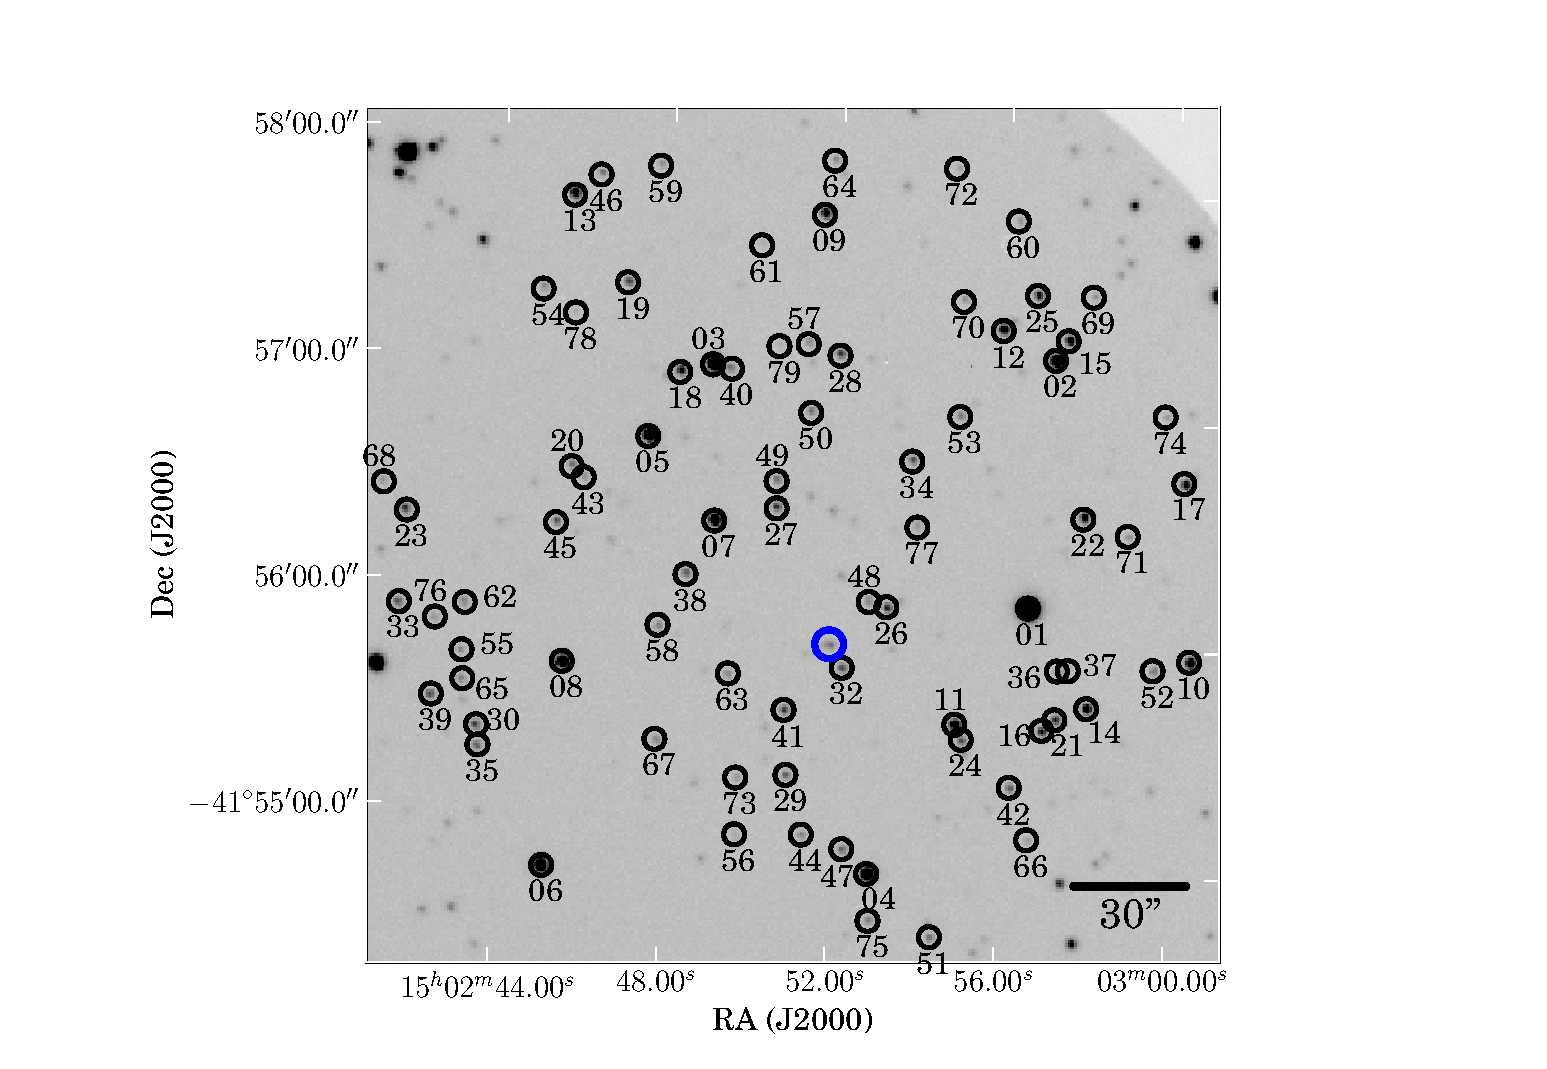
\includegraphics[width=\textwidth, trim=2cm 0 5cm 0, clip]{chapter_sn1006/plots/overview_labeled_sn1006.pdf} 
   \caption[Close-up of the candidates in SN 1006] {V-Band image taken by the 2.3~m Telescope. We have marked \candstar{31}, which was not observed due to broken fibres, with a blue circle. With the a brightness of $V=17.87$ \candstar{31} is fainter than our primary catalog ($V<17.5$~mag), and is the only star which lacks a spectrum to $V=19~\textrm{mag}$ in the remnant's centre.}
   \label{fig:sn1006:zoomed_overview}
\end{figure}


We first applied a cosmic ray removal tool on the raw 2D frames \citep{2001PASP..113.1420V}. The data was then reduced with the ESO-CPL pipeline (version 5.2.0), using the GIRAFFE instrument recipes (version 2.8.9). The only variation that was made to the default parameters was the usage of the Horne extraction algorithm instead of the "Optimal"-extraction algorithm. This yielded 366 individual spectra of the candidate stars and an additional 39 calibration star spectra. 


\section{Analysis}
\label{sec:sn1006_analysis}
\subsection{Radial Velocity}

\begin{figure}[tb] %  figure placement: here, top, bottom, or page
   \centering
   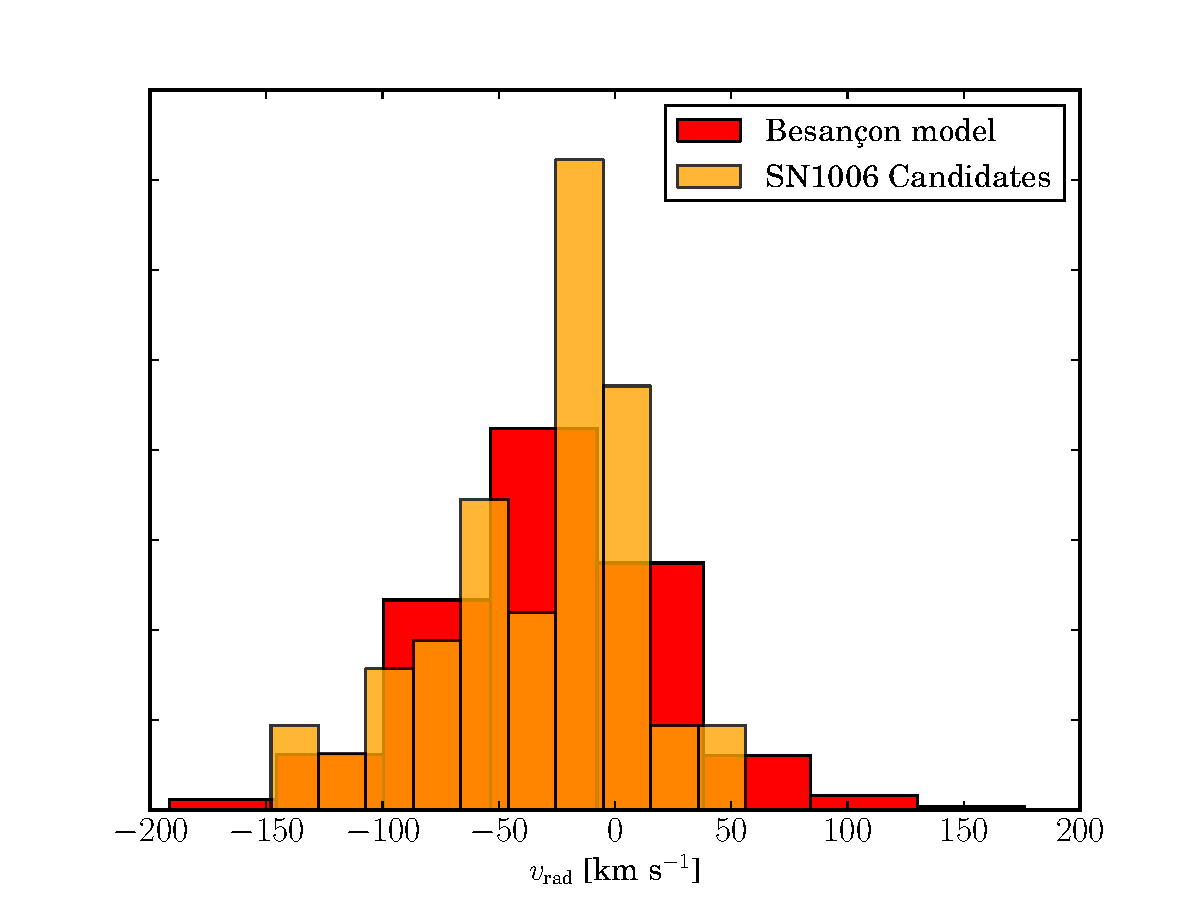
\includegraphics[width=\textwidth]{chapter_sn1006/plots/sn1006_vrad_besancon.pdf} 
   \caption[Radial velocity of all candidates in SN 1006 compared with Besan\c{c}on Model]{Comparison of all candidate stars with the distribution of stars taken from the the Besan\c{c}on kinematic model. The model input parameters were a search area of 1 square degree around the centre of \sn{1006}{} and a magnitude limit of $10<\textrm{V}<17.5$}
   \label{fig:sn1006_vrad_comp}
\end{figure}


To obtain radial velocities we employ a two step process. We used a solar spectrum from \citet{1984sfat.book.....K} with the standard cross-correlation technique described in \citet{1979AJ.....84.1511T} and implemented in the \gls{pyraf} task \textsc{fxcor}. The cross-correlation was performed on each individual spectrum. The results were then heliocentrically corrected, and then averaged for each star with a sigma clipping algorithm (see Table \ref{tab:sn1006_kinem}). We note that especially for faint objects we observe a second cross-correlation peak at 0~\kms and believe that this is reflected sun light from the moon. We believe that this has a negligible effect on our radial velocity measurement.
In Figure \ref{fig:sn1006_vrad_comp} we have compared our radial velocity measurements with the Besan\c{c}on kinematic model of the Milky way \citep{2003A&A...409..523R}. Our selection criteria for creating the  Besan\c{c}on kinematic model was all stars within 1 square degree of \sn{1006}{} and a magnitude cut of $10<\textrm{V}<17.5$. We compared the resulting 10000 stars to our 78 stars in the sample in Figure \ref{fig:sn1006_vrad_comp}. 




\subsection{Rotational Velocity}
\label{sec:sn1006_rotvel}
Due to the direction looked through the Galaxy, there is a large velocity spread in the direction of \sn{1006}{} (see Figure \ref{fig:sn1006_vrad_comp}) making it hard to isolate a \gls{donor} star based just on kinematic features. A distinguishing feature for a \gls{donor} star should be rotation (discussed in Chapter \ref{chap:sn1572_starg}), especially if the donor star isn't a giant. The rotational velocities in Chapters \ref{chap:sn1572_starg} \& \ref{chap:sn1572_hires} were all measured manually. In these previous measurements we selected weak iron lines and stacked them to obtain a line profile, which was compared to synthetically rotationally broadened lines. This was a feasible way for six spectra, it is however not feasible for more than 200 spectra. 

Measuring repetitive structures like line profiles is much more straight forward in Fourier space. The intrinsic spectrum ($f_\textrm{spectrum}$) of a star is broadened by a convolution of the intrinsic spectrum with a rotational broadening kernel ($g_\textrm{rotation}$). The next broadening is introduced by the instrument (instrumental kernel $h_\textrm{instrument}$) before being recorded on the detector. Assuming an unbroadened synthetic spectrum ($f_\textrm{synthetic}$), matching the intrinsic stellar spectrum, we can describe a convolution in Fourier space as,
\begin{align*}
	f_\textrm{observed} =& f_\textrm{spectrum} \otimes \underbrace{g_\textrm{rotation} \otimes h_\textrm{instrument}}_{f_\textrm{profile}}\\
     F(f_\textrm{spectrum} \otimes g_\textrm{rotation} \otimes h_\textrm{instrument}) =& F(f_\textrm{spectrum}) \times F(g_\textrm{rotation}) \times F(h_\textrm{instrument})\\
     \Rightarrow \frac{F(f_\textrm{observed})}{F(f_\textrm{synthetic})} \approx& F(f_\textrm{profile}),
\end{align*}
where $F$ denotes the Fourier transform. This yields the line profile which we can separate, knowing the resolution of the instrument, into an instrumental profile and a rotational kernel . This technique has been described by a selection of authors \citep[e.g.][]{1977ApJ...211..198G}. \textsc{fxcor} uses this technique to measure radial velocities from shift of the profile peak relative to rest. We have applied this technique successfully to extract the rotation for some of the stars were the quality of the spectra was adequate (see Table \ref{tab:sn1006_kinem}).


\subsection{Stellar Parameters}
\label{sec:sn1006_stelparam}

We obtained detailed stellar parameters for the donor candidates with $V<17.5$ by employing a grid based technique (three dimensional grid in \teff, \logg\ and \feh). \gls{moog} was used to synthesise the spectral grid using the model stellar atmospheres by \citet{2003IAUS..210P.A20C}. Line wings were taken into account up to 8~\AA\ away from line centre, which seemed to be a reasonable compromise between grid creation time and accuracy. For the atomic lines we merged values from the \gls{vald} with adjusted values (to reproduce the Arcturus and the Sun) from \cite{2008A&A...486..951G}. In addition, we used the measured molecular lines described in  \citet{1995KurCD..23.....K}. The final grid extends from 3500~K to 7500~K in \gls{teff} with a step size of 250~K, in \gls{logg} it ranges from  0 to 5 with a stepsize of 0.5 and in \feh\ it ranges from -2.5 to 0.5 with a stepsize of 0.5 (with an extra set of points at 0.2). 

We used the appropriate sections from the Solar spectrum \citep{1984sfat.book.....K} and the Arcturus spectrum \citep{2000vnia.book.....H} to calibrate our spectral grid. We measured stellar parameters by first finding the best fitting grid point and then using the minimizer \gls{minuit} to find a minimum by interpolating between the gridpoints \citep[described in Appendix \ref{chap:ndinterp} of this thesis;][]{Barber96thequickhull}. For the Sun we obtain stellar parameters of \teff=5825~K, \logg=4.4 and \feh=-0.12 and for Arcturus we obtain stellar parameters of \teff=4336~K, \logg=1.9, \feh=-0.67. We acknowledge the error in measurement, but believe our spectral grid to be accurate enough for distinguishing a potential donor candidate against an unrelated star. 

To measure our observed spectra we first fitted the continuum with Legendre polynomials with a maximum order of 3 and a sigma clipping algorithm discarding the lines. The order that gave the lowest \gls{rms} of the fit was used. We then combined the spectra using the previously measured \gls{vrad} and the computed heliocentric correction. In addition, we broadened the synthetic spectral grid with a rotational kernel for each star where applicable. These spectra were then fitedt using the previously described algorithm, except that we added the $B-V$ photometric temperature as a prior. As the photometric temperature uses the metallicity as an input parameter we recalculated the photometric temperature prior using the metallicity determined by the fit. This procedure was repeated until the gravity estimate converged to less than 0.1~dex. We believe our temperatures to be good to a few hundred K, our surface gravities as well as metallicities have a systematic uncertainty of roughly 0.5~dex. 

The stellar parameters can be seen, as fits to the spectra, in Figure \ref{fig:sn1006_candfit} and in tabulated form in Table \ref{tab:sn1006_stel_param}. The final set of stellar parameters shows a typical distribution of many dwarfs and a few giants. None of the stars seem to be unusual in any way. Giant stars, which are expected to have relatively low \vrot\ post explosion (but still $> 20~\kms$), are absent from the remnant's centre. 
%!TEX root = ../../thesis.tex
\ctable[
caption=SN 1006 candidates ($V<17.5$) stellar parameters,
label={tab:sn1006_stel_param},
width=\textwidth
]
{lXXXXX}{}{\FL
Name & $\teff $ & $\logg$ & \feh & 
V&\vrot \\ 
 & K & dex & dex& mag&\kms \ML
01 & 4285 & 2.0 & $-1.0$& $13.50$ &$<10$\\
02 & 4001 & 0.8 & $-1.4$& $15.37$&$<10$\\
03 & 5446 & 4.0 & $-0.6$& $15.04$&$<10$\\
04 & 5347 & 4.0 & $-0.6$& $15.47$&$<10$\\
05 & 5191 & 3.7 & $-0.6$& $15.50$&$<10$\\
06 & 5874 & 4.5 & $-0.7$& $15.50$&$<10$\\
07 & 4884 & 4.2 & $-0.8$& $15.90$&$<10$\\
08 & 5954 & 4.2 & $-0.5$& $15.86$&$<10$\\
09 & 4217 & 3.9 & $-2.5$& $16.58$&$<10$\\
10 & 5662 & 4.3 & $-0.8$& $16.30$&$10$\\
11 & 5489 & 4.1 & $-0.8$& $16.33$&$<10$\\
12 & 5313 & 4.4 & $-0.9$& $16.39$&$16$\\
13 & 5114 & 4.0 & $-0.7$& $16.49$&$<10$\\
14 & 5245 & 4.3 & $-0.7$& $16.56$&$<10$\\
15 & 5503 & 4.2 & $-0.7$& $16.63$&$<10$\\
16 & 4448 & 4.0 & $-1.8$& $17.26$&$14$\\
17 & 5515 & 4.4 & $-1.2$& $16.66$&$<10$\\
18 & 5341 & 4.1 & $-0.9$& $16.77$&$12$\\
19 & 3846 & 4.1 & $-2.4$& $17.39$&$17$\\
21 & 4510 & 3.1 & $-1.3$& $17.36$&$13$\\
22 & 6448 & 4.2 & $-0.4$& $16.71$&$13$\\
23 & 4429 & 4.0 & $-1.8$& $17.39$&$14$\\
25 & 6119 & 4.9 & $-0.7$& $17.03$&$<10$\\
26 & 5619 & 4.0 & $-1.1$& $17.23$&$<10$\\
27 & 5336 & 4.0 & $-1.3$& $17.47$&$<10$\\
28 & 5379 & 4.3 & $-1.1$& $17.43$&$<10$\\
\LL}


\section{Conclusions}
\label{sec:sn1006:conclusion}
In this work we have scrutinised all stars to a limit of $0.5~\lsun(V)$ at the distance of the \sn{1006}{}\ remnant. None of the stars scrutinised in our sample show features consistent with those expect for donor star models. 

Giant star progenitors are easily ruled out because there is no star bright enough to be at the distance of the remnant. \citet{2000ApJS..128..615M} suggests that giant donors have a luminosity of $\approx 1000~\lsun$ ($V\approx9$ at the distance of the remnant) for at least 100,000 years. Furthermore, these models suggest that the giant donor is likely to have a high temperature of more than $10^4\,K$. In addition, the star should have some rotation in excess of what has been measured for any of the stars in this sample. In summary, there is no viable giant star donor star scenario for the stars located in \sn{1006}{}. 

Sub giant donors should also be very luminous \citep{2000ApJS..128..615M} with a minimum expected luminosity of $L\approx500\,\lsun$ ($V\approx9.7$ at the distance of the remnant) lasting for 1400--11,000 years, although theoretical models allow much more larger scope for variation of this class of stars \citep{2003astro.ph..3660P}. While they might have a \gls{vrad} which could be masked by the large expected dispersion in the direction of \sn{1006}{}, the expected $\vrot\approx80\,\kms$ (see Figure \vref{fig:han2008_vrad} and Figure \ref{fig:han2008_vrot_compare}), far exceeds any star in our sample.  Therefore, we believe we can confidently rule out sub giant donor stars in this case as well. 

Finally, main sequence stars, according to \citet{2000ApJS..128..615M} are expected to have a similar brightness to sub giant stars, although this enhanced luminosity depends on the details of how energy is deposited from the explosion \citep[see][]{2003astro.ph..3660P}.  However, main sequence donors should have both substantial spatial motion coupled with very high rotation (see Figure \vref{fig:han2008_vrad} and Figure \ref{fig:han2008_vrot_compare}). No star shows any of these features in our sample, and our sample's depth should cover all conceivable post-evolutionary scenarios, even for a main sequence donor star.

There are two additional issues worthy of further discussion. Firstly, rotation can be lost due to expansion (see Section \ref{sec:sn1572_starg_rot}). This, however is a priori unlikely (priv. comm. Chris Tout), and should result in a star with a low gravity, relatively high luminosity (unless it were to become extremely cool). No such star is present in SNR 1006. Secondly, measurements by \citet[see Figure \ref{fig:sn1006_uvprobe}]{2005ApJ...624..189W}cast doubt on a precise determination of the centre. Their research suggests that the centre of the iron core is offset from the geometric centre determined by the shocked \gls{ism}. However, we argue that this does not mean that the centre of mass (where a donor star would reside) is necessarily off centre. In fact, \cite{2010ApJ...708.1703M} suggest that the iron ejecta is offset from the centre of mass, which suggests that the centre of the iron core will be different than the centre of mass. In general, explosion models are consistent with the center of  mass being given by the outer shock, not the iron core. In addition, other groups are also currently surveying \sn{1006}{} with a spatially larger but photometrically shallower field (priv. comm. Pilar Ruiz-Lapuente) and have not yet found a viable companion. In summary our research shows a consistent result to \sn{1572}{} - no identifiable donor star.

\begin{figure}[tb] %  figure placement: here, top, bottom, or page
   \centering
   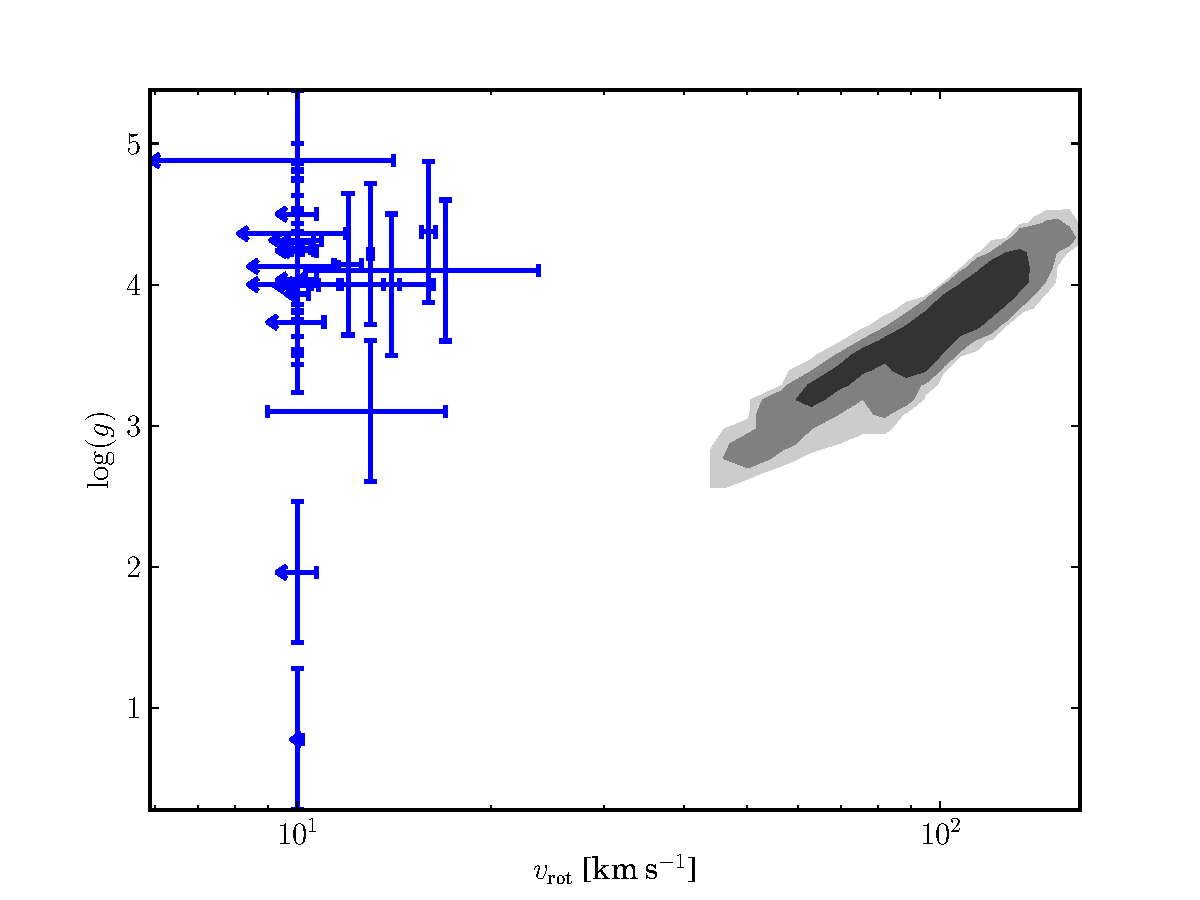
\includegraphics[width=\textwidth]{chapter_sn1006/plots/compare_vrot.pdf} 
   \caption[Comparison of rotation and surface gravity of SN 1006 candidates]{Comparison of the evolutionary state and rotational velocity of 55000 binary synthesis \glsentryname{sds} progenitors \citep[gray shades;data from][]{2008ApJ...677L.109H} with the measured rotation from this work. Due to the resolution of the spectrograph most of these stars only have an upper limit of the rotation speed of $\vrot=10~\kms$}
   \label{fig:han2008_vrot_compare}
\end{figure}


\begin{figure}[tb] %  figure placement: here, top, bottom, or page
   \centering
   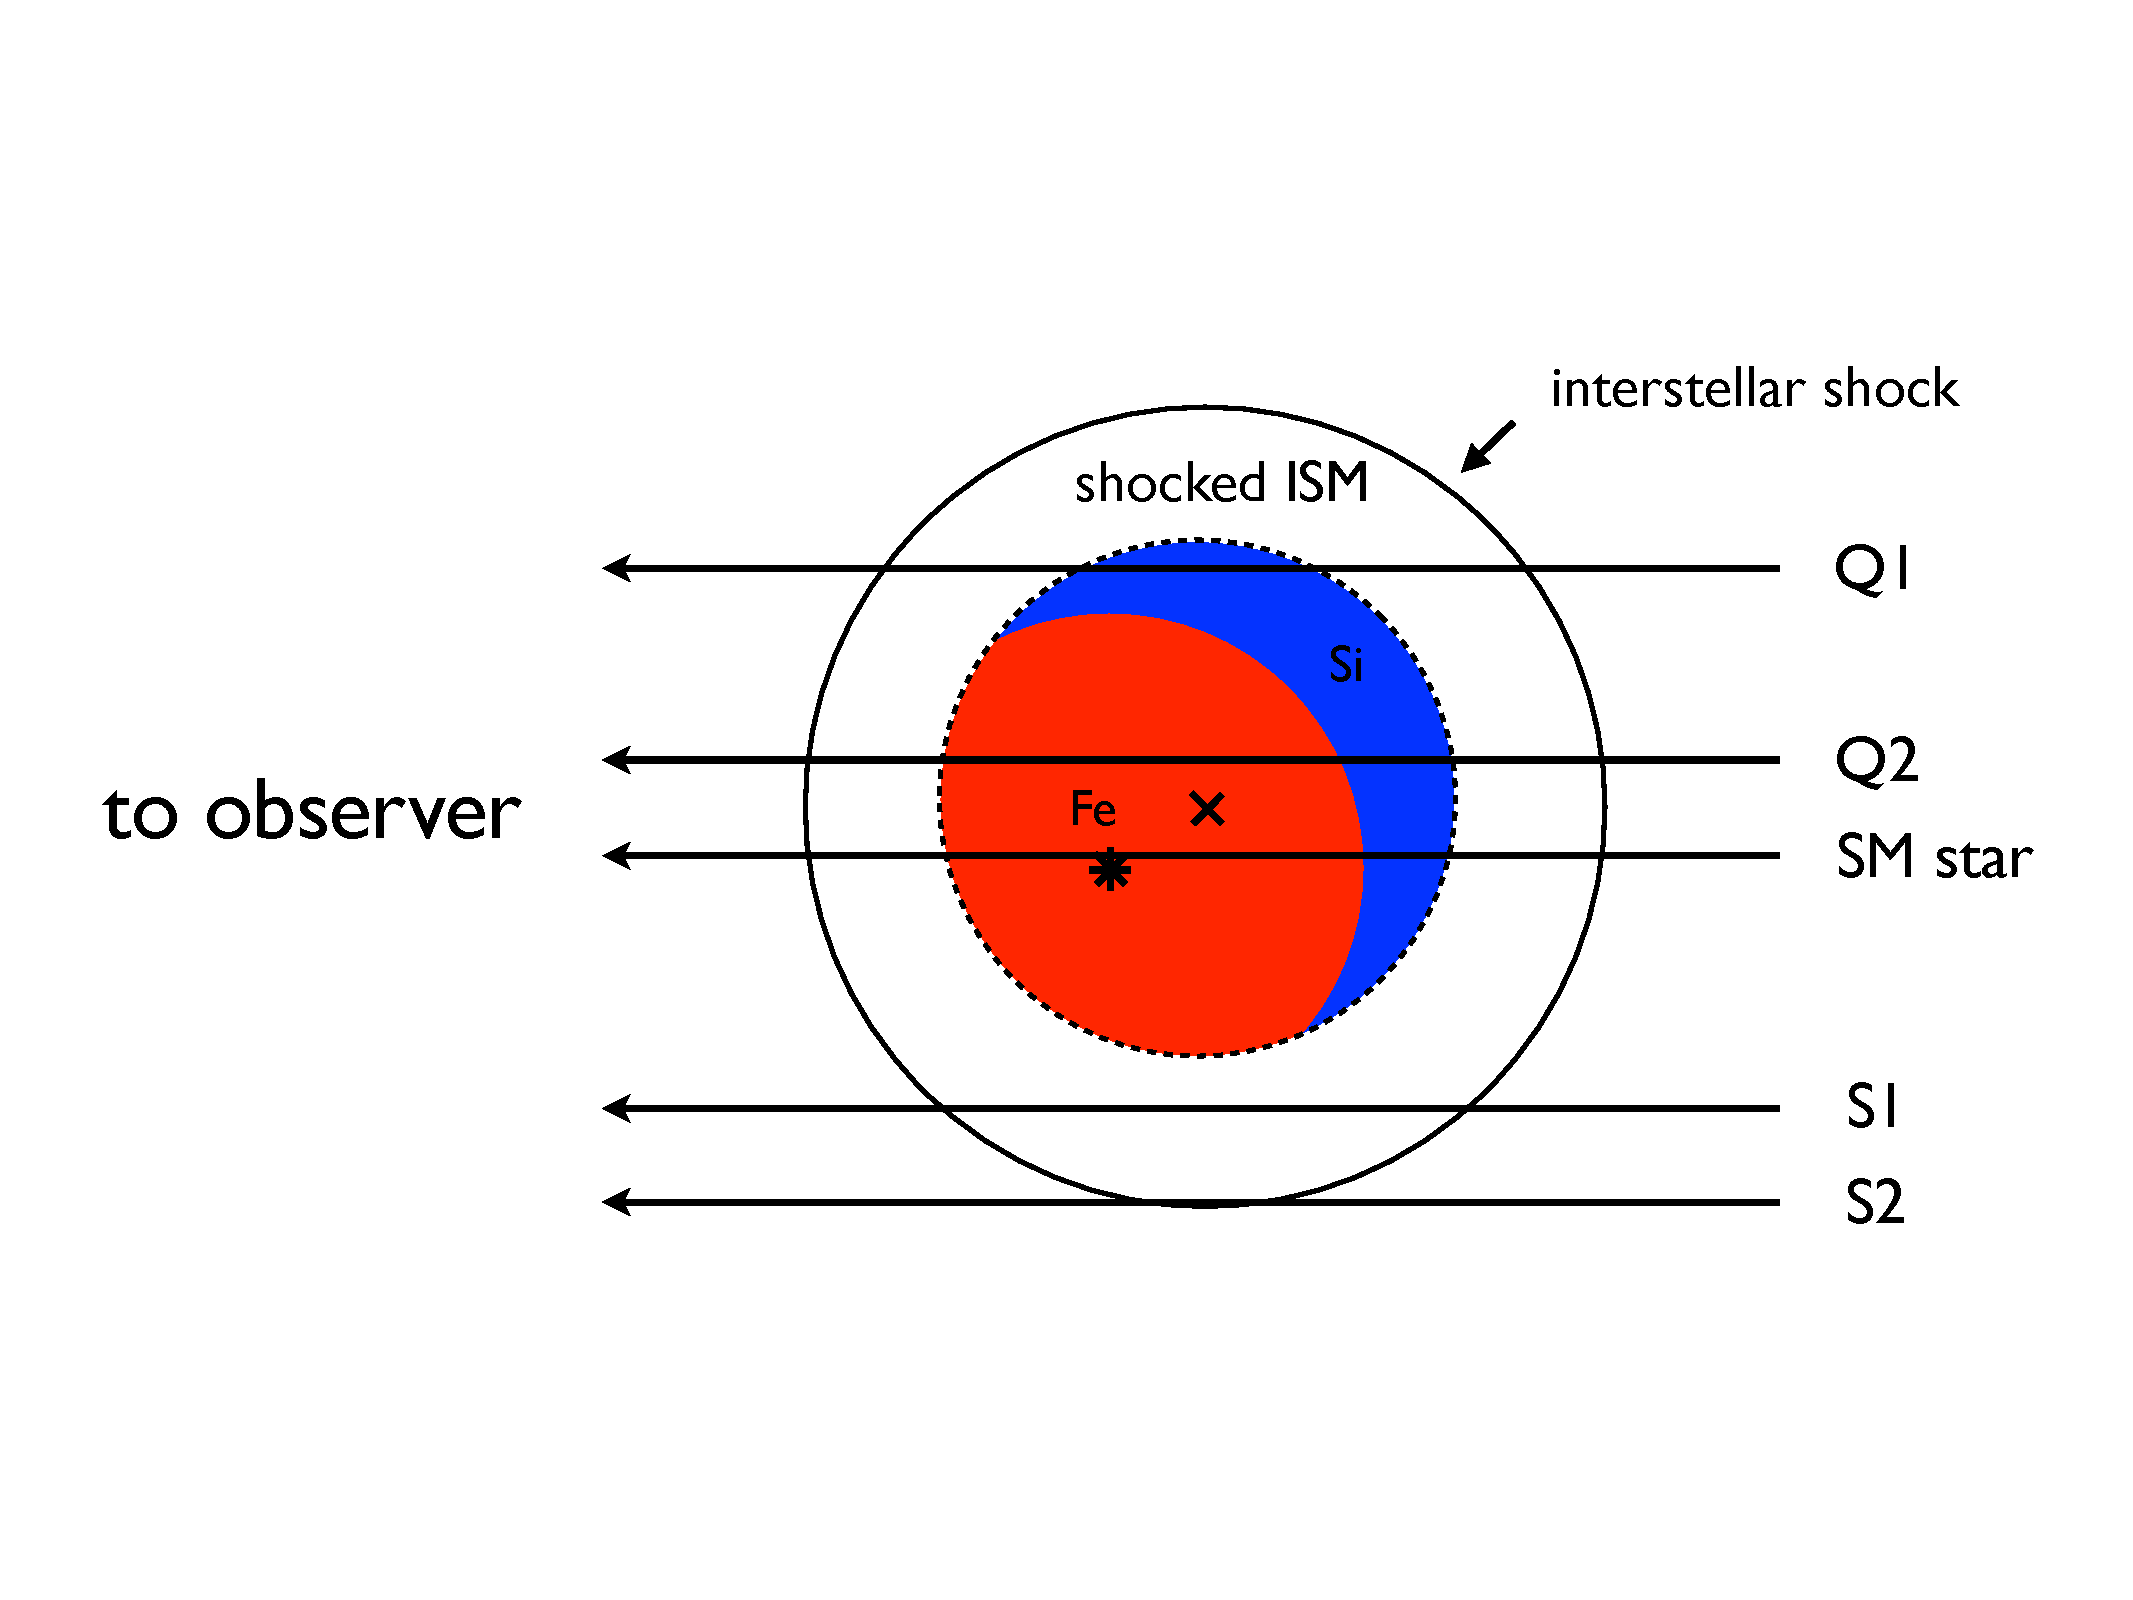
\includegraphics[width=\textwidth]{chapter_sn1006/plots/Winkler2005_probingsn1006_cropped.pdf} 
   \caption[Background UV sources probing the remnant]{Background UV sources probing the remnant. Figure adapted from \citet{2005ApJ...624..189W}}
   \label{fig:sn1006_uvprobe}
\end{figure}

The observations presented here for \sn{1006}{} are in conflict with the standard \snia\ donor star scenarios, which include accretion onto a white dwarf from a main sequence, sub giant, or giant companion. 
A few non-standard scenarios survive our observational tests. These include a helium white dwarf as a donor star (see Section \ref{sec:intro:subchandra}), which would not be detectable with our observations, although it is unlikely that a helium white dwarf would survive the explosion (priv. comm. R\"udiger Pakmor). The other possibility is that \sneia\ (or at least \sn{1006}{} and \sn{1572}{}) do not have donor stars, consistent with a \gls{dds}.

Another remnant that can be subjected to such an intensive search is Kepler (\sn{1604}). Kepler seems to be different from either \sn{1572}{} and \sn{1006}{}\ due to detection of interaction with the \gls{csm}. Observational facts of the Kepler remnant  as well as the description of the donor star search will be discussed in the conclusion of this thesis (Chapter \ref{chap:conclusion}).



%% !TEX root =../thesis.tex
\chapter{SN1006}
\label{chap:three}

\lettrine[lines=4]{L}{orem} ipsum dolor sit amet, consectetuer
adipiscing elit. Mauris posuere, elit ac suscipit pulvinar, purus
felis vehicula purus, sed pellentesque arcu nibh eu turpis. Vivamus
volutpat convallis mi. Aliquam varius magna eu urna lacinia
dignissim. Proin venenatis tellus. Fusce pede dui, semper varius,
venenatis vitae, ultrices ac, dolor. Proin diam. Suspendisse eget
purus id leo accumsan scelerisque. Integer rutrum. Etiam risus nibh,
auctor eu, eleifend id, interdum ut, odio. Suspendisse
potenti. Praesent ultricies, mauris convallis vestibulum viverra,
nulla risus porttitor tellus, ut consequat velit nunc at nisi. Nulla
rhoncus nisl quis urna. Morbi sed nunc at tortor rhoncus
iaculis. Lorem ipsum dolor sit amet, consectetuer adipiscing elit. Sed
augue. Nunc molestie.

Maecenas at lectus id nunc bibendum placerat. Suspendisse cursus,
magna vitae blandit bibendum, nisi justo facilisis mi, at faucibus
elit urna id felis. Lorem ipsum dolor sit amet, consectetuer
adipiscing elit. Maecenas risus erat, ornare ac, varius nec, molestie
sed, nulla. Praesent sem urna, sollicitudin in, vulputate at, suscipit
vehicula, lectus. Integer mollis. Curabitur ornare, erat a facilisis
sagittis, risus nulla faucibus diam, at vehicula justo magna nec
urna. Pellentesque rhoncus, turpis eu facilisis molestie, diam ipsum
tristique massa, nec auctor risus diam quis metus. Lorem ipsum dolor
sit amet, consectetuer adipiscing elit. Fusce varius iaculis
neque. Aliquam erat volutpat. Cras sit amet nisi sit amet diam
imperdiet molestie. Quisque nec nisl. Cras nisi velit, pharetra sed,
cursus nec, euismod ac, turpis.

Morbi tincidunt, tellus nec dignissim congue, risus libero
sollicitudin tellus, sit amet porta magna libero sed ante. In id orci
eget nibh ultrices ultrices. Sed feugiat lobortis augue. Integer
nulla. Phasellus lacus diam, ornare id, ornare ut, dictum non,
velit. Ut egestas, risus quis placerat fringilla, nisl nunc tincidunt
ligula, et blandit dui diam vel sem. Morbi mattis turpis et purus
pellentesque accumsan. Mauris enim massa, sollicitudin at, lobortis
quis, ultricies sed, nunc. Pellentesque habitant morbi tristique
senectus et netus et malesuada fames ac turpis egestas. In in
arcu. Vestibulum ante ipsum primis in faucibus orci luctus et ultrices
posuere cubilia Curae; Donec eleifend molestie enim. Etiam justo. Sed
pharetra ultrices lectus. Mauris imperdiet varius purus. Aliquam
commodo adipiscing est. Pellentesque vitae odio fringilla pede viverra
tempor. Vivamus sed sem. Quisque molestie elementum lorem. Proin
aliquam odio vel sapien.

Quisque urna. Praesent scelerisque tortor nec elit. Pellentesque non
urna. Duis non sapien id nunc rutrum facilisis. Donec lectus ipsum,
ullamcorper vel, sollicitudin a, tempor a, sapien. Nam dui. In hac
habitasse platea dictumst. Integer eu ligula id lacus sollicitudin
sodales. Nam aliquam nibh vitae urna gravida rutrum. Aliquam erat
volutpat. Integer gravida mattis tellus. Etiam ipsum lacus, dapibus
id, volutpat eget, vestibulum vel, pede. In odio quam, viverra id,
adipiscing nec, consequat ut, orci. Nunc sit amet neque eu risus
dictum ultrices. Proin sem quam, ullamcorper ut, posuere at, tempus
eget, nibh. Cras ipsum. Phasellus bibendum purus eu enim. In hac
habitasse platea dictumst. Praesent eget leo ac sem congue sodales.

Nunc malesuada turpis vitae neque. Donec sollicitudin libero vel
nisi. Aliquam congue sem sed est. Integer eget ipsum. Nam eu
mauris. Aliquam vehicula tempor nulla. Duis faucibus ornare
elit. Vivamus nunc. Phasellus placerat, orci non blandit scelerisque,
neque urna faucibus justo, non gravida pede sem a urna. Sed eget arcu
eget enim pellentesque tincidunt. Cum sociis natoque penatibus et
magnis dis parturient montes, nascetur ridiculus mus. In in nulla sed
est venenatis sagittis. Mauris nibh orci, adipiscing in, blandit quis,
vulputate vitae, tortor. Quisque venenatis. Ut leo quam, pellentesque
vitae, dictum ut, vestibulum at, turpis. Aliquam id urna. Vestibulum
nunc mauris, facilisis sed, molestie quis, consequat non, dui.

Duis id metus et tortor viverra varius. Vivamus consequat. Sed
bibendum ultricies lectus. Pellentesque vulputate orci vitae
augue. Vivamus dignissim pharetra mauris. Lorem ipsum dolor sit amet,
consectetuer adipiscing elit. Vestibulum purus purus, commodo in,
consequat eu, lobortis eu, sem. Proin volutpat, pede eu imperdiet
bibendum, nulla odio lobortis eros, eu aliquet neque nunc eu
enim. Donec non nunc. Aliquam erat volutpat. Ut cursus fermentum orci.

Class aptent taciti sociosqu ad litora torquent per conubia nostra,
per inceptos himenaeos. Donec ante eros, porttitor vel, pellentesque
sit amet, laoreet ut, velit. Vestibulum sit amet turpis sed lorem
vestibulum vulputate. Maecenas sed orci in ante pharetra accumsan. Sed
id nibh. Pellentesque dapibus varius neque. Pellentesque habitant
morbi tristique senectus et netus et malesuada fames ac turpis
egestas. Nullam ultrices augue. Lorem ipsum dolor sit amet,
consectetuer adipiscing elit. Etiam convallis placerat
tortor. Suspendisse potenti. Mauris porttitor, justo et mollis
dapibus, dui nunc accumsan dolor, quis sollicitudin est nisi at
libero. Donec sollicitudin eros sed neque. Nunc at quam.

Donec id arcu. Sed vel sapien sit amet metus vestibulum
fringilla. Etiam fringilla ligula at arcu. Donec bibendum sem et
quam. Nam diam mauris, malesuada vel, placerat a, fermentum sit amet,
lectus. Cras venenatis justo nec leo. Aliquam vulputate erat. Cras
turpis. Cras gravida. Aliquam erat volutpat. Sed porta pretium
ligula. Mauris viverra, nisi euismod vulputate lobortis, est tortor
consectetuer arcu, at congue quam ipsum sit amet sem. Cum sociis
natoque penatibus et magnis dis parturient montes, nascetur ridiculus
mus. Mauris eget dolor.

Suspendisse pulvinar. Suspendisse felis nisl, mattis sed, facilisis
at, laoreet vitae, magna. Suspendisse potenti. Pellentesque et ligula
vel mauris suscipit vestibulum. Phasellus eros sem, volutpat at,
feugiat ut, aliquam sed, augue. In hac habitasse platea
dictumst. Suspendisse suscipit. Cum sociis natoque penatibus et magnis
dis parturient montes, nascetur ridiculus mus. In lectus dolor,
commodo non, ultricies eu, scelerisque at, orci. Nulla
semper. Suspendisse potenti. Donec orci diam, pellentesque tristique,
tempus eget, tincidunt in, dolor. Maecenas tristique vehicula
risus. Integer vitae nisi. Aenean sed enim eu nisl suscipit
scelerisque. Integer non metus. Donec dui erat, bibendum eu, suscipit
eu, facilisis non, erat. Morbi dapibus pede id justo. Fusce lobortis
volutpat enim.

Morbi leo turpis, facilisis in, ultrices vel, adipiscing ut,
erat. Praesent ligula. Maecenas quis velit in orci adipiscing
aliquam. Quisque at pede. Integer at odio. Pellentesque feugiat tellus
sed risus. Mauris et turpis. Nam sodales. Suspendisse mollis tincidunt
sapien. In ac sapien et purus sollicitudin ultricies. Integer eget
sapien quis ligula commodo egestas. Nulla aliquam, odio sed tincidunt
blandit, pede dolor gravida nunc, nec condimentum lorem nulla eget
dui.  




%
\bibliographystyle{astroads}
\bibliography{thesis}

\end{document}
